% !TEX program = pdflatex
\documentclass{article}
\usepackage{tikz}
\usetikzlibrary{positioning,arrows.meta}
\tikzset{desk/.style={draw,rounded corners,fill=blue!8,minimum width=21mm},link/.style={-{Stealth},thick}}
\begin{document}
\section*{Routing a sample card}
\begin{figure}[ht]\centering
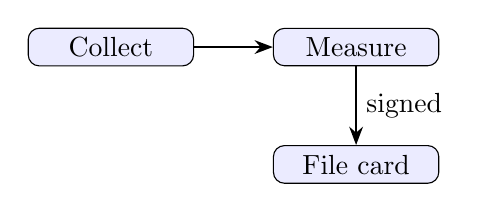
\begin{tikzpicture}

\node[desk] (a) {Collect};\node[desk,right=of a] (b) {Measure};
\node[desk,below=of b] (c) {File card};
\draw[link] (a)--(b);\draw[link] (b)--node[right]{signed}(c);
\end{tikzpicture}\caption{Cards are signed after measurement.}\end{figure}
\end{document}
